\documentclass[
11pt,notheorems,hyperref={pdfauthor=whatever}
]{beamer}
\input{loadslides.tex} % Loads packages and some defined commands
\usepackage{tikz}
\usetikzlibrary{shapes.geometric, arrows.meta, positioning, fit, backgrounds, calc, decorations.pathreplacing}


% ── Couleurs du schéma ──────────────────────────────────────────────
\definecolor{colInput}{RGB}{70,130,180}
\definecolor{colAE}{RGB}{255,165,0}
\definecolor{colMLP}{RGB}{60,179,113}
\definecolor{colCNN}{RGB}{178,34,34}
\definecolor{colLoss}{RGB}{128,0,128}
\definecolor{colOutput}{RGB}{47,79,79}
\definecolor{colBEM}{RGB}{169,169,169}
\definecolor{colLatent}{RGB}{255,215,0}
\definecolor{colLatent}{RGB}{255,245,180}
\definecolor{colLatentBorder}{RGB}{218,165,32}
\definecolor{colLatentText}{RGB}{139,69,19}
\title[
% Text entered here will appear in the bottom middle
]{Réunion du 01/06/2026}

\subtitle{IFPEN/INRIA}

\author[
% Text entered here will appear in the bottom left corner
]{
    Arthur Timbeau, 
    Adam Rozentalis,
    Julien Salomon
}


\AtBeginSection[]{
  \begin{frame}[plain]
    \vfill
    \centering
    \usebeamerfont{title}\insertsection
    \vfill
  \end{frame}
}

\begin{document}

% Generate title page

\setbeamertemplate{footline}{}
\begin{frame}
  \titlepage
\end{frame}

\setbeamertemplate{footline}{
  \hfill\insertframenumber/\inserttotalframenumber\hspace{1em}\vspace{0.5em}
}

\begin{frame}
    \tableofcontents
\end{frame}

\section{Contenu du document}

\begin{frame}{Contenu du document}
    \begin{itemize}
        \item Rappels sur les travaux précédemment réalisé et présentation des stratégies 
        \item Bref retour sur quelques approches
        \item Introduction aux nouvelles méthodes mise en oeuvre et présentation de quelques résultats
        \item Conclusion
    \end{itemize}    
\end{frame}


%%%%%%%%%%%%%%%%%%%%%%%%%%%%%%%%%%%%%%%%%%%%%%%%%%%%%%%%%%%%%%%%%%%%%%%%%%%%%%%%%%%%%%%%%%%%%%%%%%%%%%%%%%%%%%%%%%%%%%%%%%%%%
%%%%%                                   Rappels sur les stratégies employés                                             %%%%% 
%%%%%%%%%%%%%%%%%%%%%%%%%%%%%%%%%%%%%%%%%%%%%%%%%%%%%%%%%%%%%%%%%%%%%%%%%%%%%%%%%%%%%%%%%%%%%%%%%%%%%%%%%%%%%%%%%%%%%%%%%%%%%


\section{Rappels sur la stratégie globale G}

\subsection{Correction globale}

\begin{frame}{Correction globale}
    \begin{center}
    \begin{itemize}
    \item Les corrections \textbf{globales} (G) : les \textcolor{red}{rayons} et les \textcolor{blue}{azimuts}  sont fixés
    \end{itemize}
\end{center}
\end{frame}

\begin{frame}{Approche G}

Approche globale : inférences sur les efforts sur toute les sections de la pale et tous les azimuts.

    \vspace{0.3cm}

    \begin{columns}[c]
        \column{0.44\textwidth}
        \textbf{Inputs :}
        \begin{itemize}\small
            \item Vitesse de rotation $\Omega \in \mathbb{R}$
            \item Vitesse freestream $U_{\infty} \in \mathbb{R}$
            \item Yaw $\gamma \in \left[-\frac{\pi}{4}, \frac{\pi}{4}\right]$
        \end{itemize}

        \column{0.10\textwidth}
        \centering
        
\begin{tikzpicture}
            \draw[-stealth, line width=4pt, color=blue!70]
                (0, 0) -- (0.9, 0);
        \end{tikzpicture}

        \column{0.44\textwidth}
        \textbf{Outputs :}
        \begin{itemize}\small
            \item Force normale $F_N \in \mathbb{R}^{n \times p}$
            \item Force tangentielle $F_T \in \mathbb{R}^{n \times p}$
        \end{itemize}
    \end{columns}    
\end{frame}


\begin{frame}{Résumé}
    \begin{itemize}
        \item \centering  $G$ :     inputs = $(\Lambda)$                || outputs = $(\mathbf{F_n}, \mathbf{F_t}) \in \mathbb{R}^{2np}$
    \end{itemize}

     \vspace{0.3cm}

     Où $\Lambda$ est un vecteur contenant d'autres paramètres indépendant de la géométrie et de la discrétisation.
\end{frame}

\subsection{Approche directe/intermédiaire}

\begin{frame}{Approche directe}
    \textbf{Approche directe} : corriger directement les efforts retournés par la BEM : 
    
    \vspace{0.4cm}
    \begin{center}
    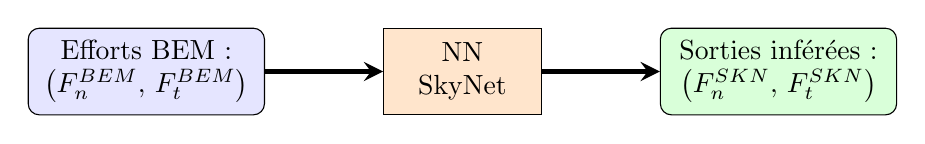
\begin{tikzpicture}[node distance=1.5cm]
        \node[draw, rounded corners, fill=blue!10, minimum width=3cm, minimum height=1.1cm, align=center]
            (bem) {Efforts BEM : \\ $\bigl(F_n^{BEM},\, F_t^{BEM}\bigr)$};
        \node[draw, fill=orange!20, minimum width=2cm, minimum height=1.1cm, align=center, right=1.5cm of bem]
            (nn)  {NN\\SkyNet};
        \node[draw, rounded corners, fill=green!15, minimum width=3cm, minimum height=1.1cm, align=center, right=1.5cm of nn]
            (skn) {Sorties inférées : \\ $\bigl(F_n^{SKN},\, F_t^{SKN}\bigr)$};
        \draw[-stealth, line width=2pt] (bem) -- (nn);
        \draw[-stealth, line width=2pt] (nn)  -- (skn);
    \end{tikzpicture}
    \end{center}

    Dans ce cas, le vecteur $\Lambda$ contient les efforts normaux calculés par la BEM (soit une valeur, soit un distribution radiale ou azimutale ou soit 
    une matrice de $n\times p$ coefficients.)
\end{frame}

\begin{frame}{Approche intermédiaire}
    Approche intermédiaire : considérer une variable en amont des efforts (présente dans BEM et FWV) et inférer dessus. 

        \begin{center}
    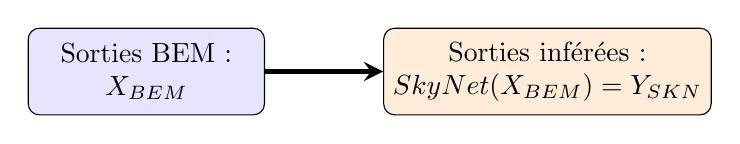
\begin{tikzpicture}[node distance=1.5cm]
        \node[draw, rounded corners, fill=blue!10, minimum width=3cm, minimum height=1.1cm, align=center]
            (bem) {Sorties BEM : \\ $X_{BEM}$};
        \node[draw, rounded corners, fill=orange!15, minimum width=3cm, minimum height=1.1cm, align=center, right=1.5cm of bem]
            (var_inter) {Sorties inférées : \\ $\text{SkyNet}(X_{BEM}) = Y_{SKN}$};

        \draw[-stealth, line width=2pt] (bem) -- (var_inter);
    \end{tikzpicture}

    \vspace{0.3cm}
    Où $G$ représente les différentes formules permettant de calculer les efforts à partir de la variable inférée.

    \vspace{0.2cm}

    Par exemple, les deux modèles utilisent dans le calcul des efforts la \textbf{vitesse effective} couplé à \textbf{l'angle d'attaque}.
    \begin{columns}[c]
        \column{0.44\textwidth}
        \textbf{BEM :}
        Au niveau de la section de rayon $r$
        \begin{itemize}\small
            \item vitesse effective : $V_{eff} = \sqrt{\left[ U_{\infty}(1-a)^2 + ^\Omega r(1+a')^2\right]}$
            \item angle d'attaque : $\alpha = \varphi -\left(\beta + \theta_{pitch}\right)$
        \end{itemize}

        \column{0.10\textwidth}
        \centering
        
\begin{tikzpicture}
            \draw[-stealth, line width=4pt, color=blue!70]
                (0, 0) -- (0.9, 0);
        \end{tikzpicture}

        \column{0.44\textwidth}
        \textbf{FWV :}
        Au niveau de la section de rayon $r$ 
        \begin{itemize}\small
            \item Biot-Savart :  $V_{eff} = \frac{\Gamma(||r_1|| + ||r_2||)(r_1 \times r_2)}{4\pi ||r_1|| \, ||r_2||(||r_1||\,||r_2|| + (r_1 | r_2))}$
            \item angle d'attaque :  $\alpha = \text{arctan}\bigl(\frac{(u|N)}{(u|T)}\bigr)$
        \end{itemize}
    \end{columns}    
    \end{center}
\end{frame}

\begin{frame}{Variables d'entrée}
    Que ce soit pour la variante intermédiaire ou directe, les variables d'entrées de ces modèles peuvent contenir des entrées BEM 
    \begin{itemize}
        \item Sous la forme d'une matrice de $n \times p$ coefficients dans l'approche $G$ (soit $ \Lambda \in \mathbb{R}^{2np}$)
    \end{itemize}
\end{frame}

\begin{frame}{Stratégies sans BEM : créer un challenger}
    \begin{center}
    En parallèle, des modèles émulant directement FWV (sans utiliser d'autre modèle) sont écrits dans le but de challenger les modèles corrigeant la BEM.\\ 
    Objectif : \textbf{Montrer qu'un réseau de neurones informés par un modèle physique performe mieux qu'un modèle non informé}.
    \end{center}
\end{frame}

%%%%%%%%%%%%%%%%%%%%%%%%%%%%%%%%%%%%%%%%%%%%%%%%%%%%%%%%%%%%%%%%%%%%%%%%%%%%%%%%%%%%%%%%%%%%%%%%%%%%%%%%%%%%%%%%%%%%%%%%%%%%%
%%%%%                                   Update                                                                          %%%%% 
%%%%%%%%%%%%%%%%%%%%%%%%%%%%%%%%%%%%%%%%%%%%%%%%%%%%%%%%%%%%%%%%%%%%%%%%%%%%%%%%%%%%%%%%%%%%%%%%%%%%%%%%%%%%%%%%%%%%%%%%%%%%%

\section{Update}

\subsection{Abandon de certaines stratégies}
\begin{frame}{Abandon de certaines}
    Les modèles autres que $G$ ont été mis de côté pour l'instant. 
    \begin{itemize}
    \item $G_r$ et $G_{\theta}$ du fait de leurs performances ou trop mauvaises ou trop suspecte
    \item $L$ du fait du manque de paramètres et de généralisation de notre paradigme. 
    \item Approche globale via les GBM (arbre de décision).
    \end{itemize} 
\end{frame}

\subsection{Modifications de l'approche des vitesses}

\begin{frame}{Modification de l'approche des vitesses}
    L'approche des vitesses a également été modifiée. Les variables $(V_eff, \alpha )$ sont exprimées dans une base base polaire, ce
    qui peut poser des problèmes de continuité, notamment en $\alpha = 0$. 
    
    \vspace{0.3cm}

    Ainsi, le choix s'est porté sur une expression dans une base cartésienne de ces paramètres, exprimé dans une base \textbf{(n,t)} qui s'écrit
    \[
        (a_n, a_t) = \frac{V_{eff}}{V_{app}}(\sin(\alpha), \cos(\alpha))
    \]
\end{frame}
%%%%%%%%%%%%%%%%%%%%%%%%%%%%%%%%%%%%%%%%%%%%%%%%%%%%%%%%%%%%%%%%%%%%%%%%%%%%%%%%%%%%%%%%%%%%%%%%%%%%%%%%%%%%%%%%%%%%%%%%%%%%%
%%%%%                                   GM & GV                                                                         %%%%% 
%%%%%%%%%%%%%%%%%%%%%%%%%%%%%%%%%%%%%%%%%%%%%%%%%%%%%%%%%%%%%%%%%%%%%%%%%%%%%%%%%%%%%%%%%%%%%%%%%%%%%%%%%%%%%%%%%%%%%%%%%%%%%


\section{Description des modèles}

\subsection{Introduction}

\begin{frame}{Introduction}
    L'approche globale à été décliné en 2 nouvelles approches : 
    \begin{itemize}
        \item Celle d'avant
        \item Une issue du \textit{Computer Vision}
    \end{itemize}
\end{frame}

\subsubsection{Globale Vectoriel}

\begin{frame}{GV}
    L'approche \textcolor{blue}{G}lobale-\textcolor{blue}{V}ectorielle (\textcolor{blue}{GV}) est un MLP prenant en 
    entrée un couple yaw/tsr et éventuellement des informations BEM pour prédire un  vecteur de $5184 \text{ }(= 36 \times 72 \times 2)$ dimensions
    décrivant la répartition des variables cibles sur la grille azimuth/rayon. 

    \vspace{0.3cm}

    Il s'agit essentiellement de l'approche globale connue jusqu'à maintenant.
\end{frame}

\begin{frame}{Architecture des GV}
    Les MLP ont une architecture identique à ceux d'avant, à la différence près qu'une compression
    par un auto-encodeur de la dimension est utilisé afin d'accélérer la procédure d'entraînement 
    (on diminue le coût de l'entrainement sur les $2592 \times 2$ dimensions avec un auto-encodeur
    entraîné en amont pour réduire la dimension).
\end{frame}

\subsubsection{Globale Matricielle}

\begin{frame}{GM}
    L'approche \textcolor{blue}{G}lobale-\textcolor{blue}{M}atricielle (\textcolor{blue}{GM}) consiste en la prédiction de deux matrices de taille
    $36 \times 72$ décrivant elles aussi la distribution des variables cibles sur la grille. La différence fondamentale entre les
    deux est l'approche employée : le prédicateur n'est plus un MLP mais un CNN (\textit{Convolution Neural Network}).

    \vspace{0.3cm}

    L'analogie avec le computer vision est la suivante : Il s'agit de prédire/générer une image de $36 \times 72$ pixels. 
    Chaque élément du dataset est alors vu comme 2 images (une pour $F_n \text{ et } F_t$ ou $V_{eff} \text{ et } \alpha$) de $36 \times 72$ pixels.
    Le TSR et le yaw sont considérés commme des canaux sur lesquels sont décomposés les images.  
\end{frame}

\begin{frame}{architecture des GM}
    L'architecture du CNN se construit comme suit : 
    
    \vspace{0.2cm}

    \textbf{(I)} - Une première couche de padding est appliquée pour contrôler les valeurs au bord de l'images. Elle permet, entre autres, de contrôler la périodicité dans la dimension azimutale.

    \vspace{0.2cm}

    \textbf{(II)} - Ensuite est appliqué une couche de convolution en 2 dimensions, avec un noyau de taille $3 \times 3$.

    \vspace{0.2cm}

    \textbf{(III)} - On normalise la sortie de la couche de convolution puis elle passe dans un perceptron avec une ReLU comme fonction d'activation.

    \vspace{0.2cm}

    \textbf{(IV)} - Une couche de padding est réappliquée à la sortie de la couche et est reconvertie en la sortie voulue.

    \vspace{0.3cm}

    Une couche de \textit{pooling} a également été mobilisée pour répondre à des problèmes de mémoires GPU rencontrés lors des entraînements.
\end{frame}



\subsection{Modèles de puissances}

\begin{frame}{Variante des modèles de puissances}
    Jusqu'ici, les modèles étaient conçus pour retourner une réponse optimale sur les efforts ou bien
    sur une variable antérieure à ces derniers (induction axiales, vitesse effective, etc).
    
    \vspace{0.3cm}

    Une autre approche a été expérimentée : entraîner des modèles à retourner une réponse optimale sur un produit postérieur aux calculs des efforts : la puissance. 
\end{frame}

\begin{frame}{Classe des modèle de puissance}
\begin{itemize}
    \item $\textcolor{blue}{DP}$ : MLP classique associant à un coeffcient de puissance BEM une réponse supposée ressemblante à un coefficient de puissance calculé avec SVEN : 
    \[
       Minimiser \;\; \frac{1}{n}\sum_{i = 1}^{n}|\int dP_{NN}^i - \int dP_{SVEN}^i|^2
    \]

    \item $\textcolor{blue}{GVP}$ : MLP analogue aux modèles $GV$ : prends un champs de force BEM en entrée et retourne une densité de puissance comparable à celle calculé avec SVEN pour les mêmes conditions physiques
    \[
        Minimiser \;\; \frac{1}{n}\sum_{i = 1}^{n}|P^i_{NN} - P^i_{SVEN}|
    \]
    \item $\textcolor{blue}{GMP}$ : CNN analogue aux $GM$ et retournant le même produit que les GVP
\end{itemize}
\end{frame}

\subsection{Compression et Auto-encodeurs}

\begin{frame}{Introduction}
    \begin{center}
        La mise en place de techniques de compression des données d'entrées ont également été expérimentés.
    \end{center}
\end{frame}

\begin{frame}{Auto-encodeur adapté aux \textbf{MLP}s}
    L'AE (Auto-Encodeur) vectoriel est un MLP classique qui dispose d'une fonction d'encodage vers un espace de dimension $d$ et d'une fonction de décodage dans un espace de dimension $2N_{\theta}N_r$.
    
    \vspace{0.3cm}
    
    \begin{itemize}
        \item Encodeur : $\mathbb{R}^{2N_{\theta}N_r} \rightarrow \mathbb{R}^{512} \rightarrow \mathbb{R}^{128} \rightarrow \mathbb{R}^d$
        \item Décodeur : $\mathbb{R}^d \rightarrow \mathbb{R}^{128} \rightarrow \mathbb{R}^{512} \rightarrow \mathbb{R}^{2N_{\theta}N_r}$
    \end{itemize}
\end{frame}

\begin{frame}{Auto-encodeur adapté aux \textbf{CNN}s}
    \begin{center}
        L'AE matriciel est adapté aux entrées supportées par les modèles GM. Un \textit{stride} (comprendre écart entre chaque bloc de l'image sur lesquels on convole) de 2 pixels est appliquées, sur un réseau d'une 
        profondeur de $2\text{, } 3 \text{ ou } 4$ permettant donc de réduire la taille de l'image. Une fois l'image suffisamment réduite, les canaux sont tous applatis et projeté dans un espace de dimension plus petite que celle de base.
        
        \vspace{0.3cm}
        
        L'idée est identique aux AE-GV : on dispose d'un encodeur et d'un décodeur et on entraîne le modèle à retourner une image identique à celle initiale.
    \end{center}
\end{frame}


\subsubsection{Compression à droite}
\begin{frame}{Composition à droite}
    On note $\mathcal{AE}$ un auto-encodeur de nature quelconque et $\mathcal{P}$ un prédicateur. La composition/compression à droite consiste à compresser — à projeter — l'entrée BEM vers un espace de dimension plus petite. Cette opération peut se lire de la manière suivante :
    \[
    \text{Compression à droite : }  \mathcal{P} \circ \mathcal{AE} (X_{BEM}) = X_{P} \in \mathbb{R}^{d}
    \]

    Et dans ce cas, le prédicateur $\mathcal{P}$ retourne un vecteur de l'espace latent, qui est ensuite décodé en effort SVEN.
\end{frame}

\subsubsection{Compression par le prédicateur}

\begin{frame}{Encodage par le prédicateur}
    Avec les mêmes notations, la composition/compression à gauche consiste à intégrer la procédure d'encodage dans le prédicateur $\mathcal{P}$, ce qui peut s'écrire symboliquement 
    \[
        \text{Compression à gauche : } \mathcal{P}(X_{BEM}) = X_{P} \in \mathbb{R}^d
    \]

    Le prédicateur $\mathcal{P}$ fait directement partie de l'encodage, et l'auto-encodeur sert à revenir dans l'espacede pleine dimension.
\end{frame}



\begin{frame} {Shéma descriptif des modèles}
    \tiny
    \begin{figure}
    \resizebox{\linewidth}{!}{%
    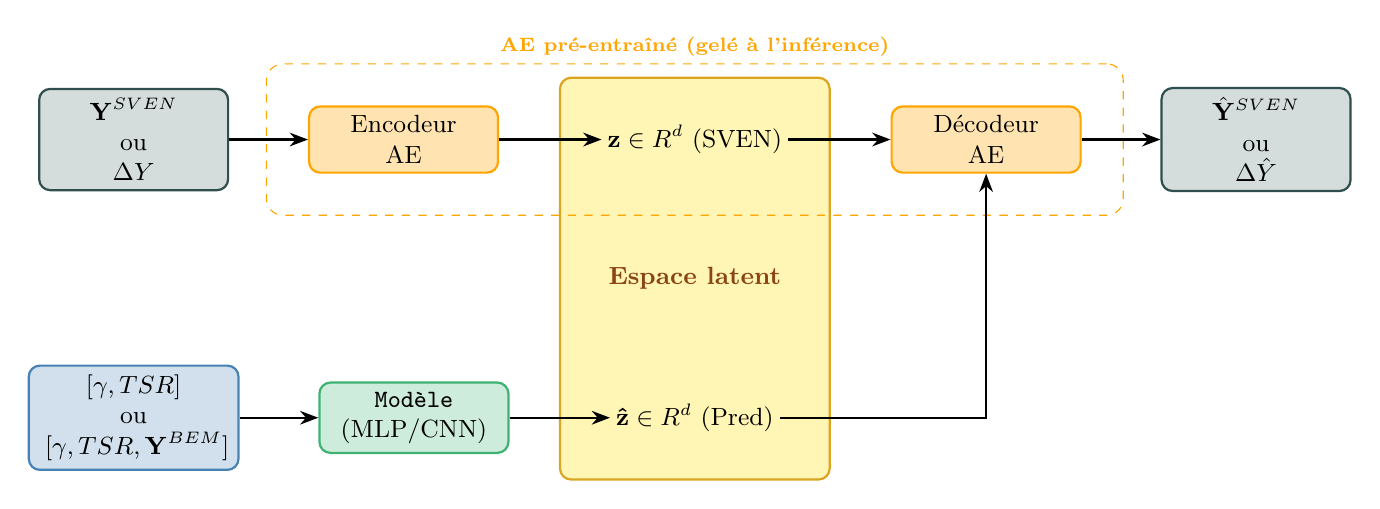
\begin{tikzpicture}[
            font=\small,
            node distance=1.2cm and 1.2cm,
            box/.style={rectangle, rounded corners=4pt, minimum width=2.4cm, minimum height=0.8cm, text centered, draw, thick, align=center},
            lat/.style={rectangle, text centered, draw=none, fill=none, inner sep=2pt},
            arrow/.style={-Stealth, thick},
            lbl/.style={font=\footnotesize\itshape, text=gray}
        ]

        %% ── LIGNE 1 : SVEN / AE ──────────────────────────
        \node[box, fill=colOutput!20, draw=colOutput] (sven_in) {$\mathbf{Y}^{\text{SVEN}}$ \\ ou \\ $\Delta Y$};
        \node[box, fill=colAE!30, draw=colAE, right= 1cm of sven_in] (enc) {Encodeur\\AE};

        \node[lat, right=1.3cm of enc] (z) {$\mathbf{z} \in \mathbb{R}^d$ (SVEN)};
        \node[box, fill=colAE!30, draw=colAE, right=1.3cm of z] (dec) {Décodeur\\AE};
        \node[box, fill=colOutput!20, draw=colOutput, right= 1cm of dec] (sven_out) {$\hat{\mathbf{Y}}^{\text{SVEN}}$ \\ ou \\ $\Delta\hat{Y}$};

        % Flèches de la ligne 1 (Horizontales)
        \draw[arrow] (sven_in) -- (enc);
        \draw[arrow] (enc) -- (z);
        \draw[arrow] (z) -- (dec);
        \draw[arrow] (dec) -- (sven_out);


        %% ── LIGNE 2 : Modèle prédictif ───────────────────────────────────────
        \node[box, fill=colInput!25, draw=colInput, below=2.2cm of sven_in] (x_in)
            {$[\gamma,\text{TSR}]$\\ ou \\ $\;[\gamma,\text{TSR},\mathbf{Y}^{\text{BEM}}]$};
            
        \node[box, fill=colMLP!25, draw=colMLP, right= 1cm of x_in] (model)
            {\texttt{Modèle}\\(MLP/CNN)};

        \node[lat] (z_hat) at (z |- model) {$\mathbf{\hat{z}} \in \mathbb{R}^d$ (Pred)};


        %% ── FLÈCHES ET RACCORDS ────────────────────────────────────
        \draw[arrow] (x_in) -- (model);
        \draw[arrow] (model) -- (z_hat);
        \draw[arrow] (z_hat.east) -| (dec.south);


        %% ── BLOC JAUNE : ESPACE LATENT ─────────────────────────────────────
        \begin{scope}[on background layer]
        \node[rectangle, rounded corners=4pt,
                fit=(z)(z_hat),
                fill=colLatent, draw=colLatentBorder, thick,
                inner xsep=15pt, inner ysep=15pt] (latent_block) {};
                

        \node[font=\small\bfseries, text=colLatentText] at (latent_block.center) {Espace latent};
        \end{scope}


        %% ── ENCADRÉ GLOBAL : AE PRÉ-ENTRAÎNÉ ─────────────────
        \begin{scope}[on background layer]

        \node[draw=colAE, dashed, rounded corners=6pt, inner sep=15pt,
                fit=(enc)(z)(dec),
                label={[font=\scriptsize\bfseries, text=colAE, yshift=-1pt]above:{AE pré-entraîné (gelé à l'inférence)}}] {};
        \end{scope}

        \end{tikzpicture}}
        \caption{Architecture générique des modes 0, 1 et 2 avec Auto-Encodeurs.}
        \label{fig:strategies_overview_final}
\end{figure}
\end{frame}


\section{Fonctions de perte}

\subsection{Description formelle}

\begin{frame}{Introduction}
    Une métrique a été utilisé afin d'améliorer les modèles optimisant
    par rapport à la vitesse et à l'angle d'attaque. L'idée de cette métrique a été poussé 
    afin de pouvoir prendre en compte le calcul une \textit{mesure de puissance} (noté $dQ$) et une \textit{mesure de poussée} (noté $dT$)\footnote{le terme \textit{mesure} est à comprendre au sens de la théorie de la mesure}.
    
    \vspace{0.2cm}

    L'idée est la suivante : au lieu de ne minimiser que la précision du calcul des vitesses, on optimise une combinaison convexe
    des vitesses et de la force et la puissance :
    \[
        \mathcal{L} = \lambda_1\mathcal{L}_1 + \lambda_2\mathcal{L}_2 + \lambda_3\mathcal{L}_3
    \]
    avec $\lambda_1 + \lambda_2 + \lambda_3 = 1$.
\end{frame}

\begin{frame}{$\mathcal{L}_1$}
    Ce terme représente (de manière relative et locale) la \textbf{puissance} et la \textbf{poussée} : 
    \[
    \mathcal{L}_1 = \frac{1}{N}\sum_{i=1}^N \Big(\frac{\hat{C}_{p}^i - C_p^i}{C_p^i}\Big)^2 + \frac{1}{N}\sum_{i=1}^N \Big(\frac{\hat{C}_{t}^i - C_t^i}{C_t^i}\Big)^2
    \]

\end{frame}

\begin{frame}{$\mathcal{L}_2$}
    Ce terme ci représente les \textbf{efforts} : 
    \begin{itemize}
        \item Option A (Erreur relative globale) : \[
            \mathcal{L}_2^A =  \frac{1}{N}\sum_{i=1}^N \Big(\frac{\hat{F}_{n}^i - F_n^i}{\max(| F_n^i |, 1)}\Big)^2 + \frac{1}{N}\sum_{i=1}^N  \Big(\frac{\hat{F}_{t}^i - F_t^i}{\max(|F_t^i|,1)}\Big)^2
        \]
        (\textbf{Nota Bene : } Le choix du dénominateur est arbitraire et a pour but d'éviter les divisions par 0)
        \item Option B (Normalisation physique globale) : \[
            \mathcal{L}_2^B =  \frac{1}{N}\sum_{i=1}^N \Big(\frac{\hat{F}_{n}^i - F_n^i}{ D^i }\Big)^2 + \frac{1}{N}\sum_{i=1}^N  \Big(\frac{\hat{F}_{t}^i - F_t^i}{D^i}\Big)^2
        \]
        où $D^i = \frac{\rho V_{app}^i |c(r_i)|}{2}$
    \end{itemize}
\end{frame}

\begin{frame}{$\mathcal{L}_3$}
    Enfin, ce terme représente \textbf{vitesses} :
    \begin{itemize}
        \item Option A (Erreur relative locale dans l'espace normalisé) :\[
            \mathcal{L}_3^A =  \frac{1}{N}\sum_{i=1}^N \Big(\frac{\hat{a}_{n}^i - a_n^i}{| a_n^i |}\Big)^2 + \frac{1}{N}\sum_{i=1}^N  \Big(\frac{\hat{a}_{t}^i - a_t^i}{|a_t^i|}\Big)^2
        \]
        \item Option B (MSE dans l'espace normalisée) :\[
            \mathcal{L}_3^B = \frac{1}{N}\sum_{i=1}^N  \Big( \hat{a}_{n}^i - a_n^i \Big)^2 + \sum_{i=1}^N  \Big( \hat{a}_{t}^i - a_t^i \Big)^2
        \]
    \end{itemize}
    Où $a$ représente une sortie (ou une étiquette) dans l'espace normalisé.
\end{frame}

\begin{frame}{Comparaison Puissance/Forces/Vitesses}
    L'objectif est de savoir laquelle des stratégies est la plus efficace :
    \begin{itemize}
        \item Effectuer une prédiction directement sur une variable d'intérêt.
        \item Effectuer une prédiction sur une variable antérieur qui aboutit au calcul de la variable d'intérêt.
    \end{itemize}
\end{frame}

\subsection{Schéma}

\begin{frame}{Schémas des fonctions de pertes}
    \begin{figure}[ht]
\centering
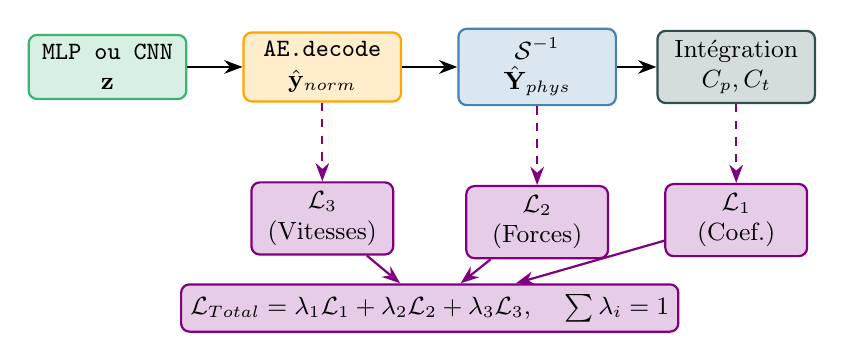
\begin{tikzpicture}[
    font=\small,
    node distance=0.5cm and 0.7cm,
    box/.style={rectangle, rounded corners=3pt, minimum width=2.0cm, minimum height=0.65cm, text centered, draw, thick, align=center},
    arrow/.style={-Stealth, thick},
    loss/.style={rectangle, rounded corners=3pt, minimum width=1.8cm, minimum height=0.6cm, text centered, draw, thick, align=center, fill=colLoss!20, draw=colLoss}
]

\node[box, fill=colMLP!20, draw=colMLP] (net) {\texttt{MLP ou CNN}\\$\mathbf{z}$};
\node[box, fill=colAE!20, draw=colAE, right=0.7cm of net] (dec) {\texttt{AE.decode}\\$\hat{\mathbf{y}}_{\text{norm}}$};
\node[box, fill=colInput!20, draw=colInput, right=0.7cm of dec] (denorm) {$\mathcal{S}^{-1}$\\$\hat{\mathbf{Y}}_{\text{phys}}$};

\node[loss, below=1.0cm of dec] (l3) {$\mathcal{L}_3$\\(Vitesses)};
\node[box, fill=colOutput!20, draw=colOutput, right=0.5cm of denorm] (integ) {Intégration\\$C_p, C_t$};
\node[loss, below=1.0cm of integ] (l1) {$\mathcal{L}_1$\\(Coef.)};
\node[loss, below=1.0cm of denorm] (l2) {$\mathcal{L}_2$\\(Forces)};

\coordinate (mid_l2_l3) at ($(l2)!0.5!(l3)$);
\node[loss, below=0.8cm of mid_l2_l3] (ltot) {$\mathcal{L}_{\text{Total}} = \lambda_1 \mathcal{L}_1 + \lambda_2 \mathcal{L}_2 + \lambda_3 \mathcal{L}_3$, \quad $\sum \lambda_i = 1$};


\draw[arrow] (net) -- (dec);
\draw[arrow] (dec) -- (denorm);
\draw[arrow] (denorm) -- (integ);

\draw[arrow, dashed, colLoss] (dec) -- (l3);
\draw[arrow, dashed, colLoss] (denorm) -- (l2);
\draw[arrow, dashed, colLoss] (integ) -- (l1);

\draw[arrow, colLoss, thick] (l1) -- (ltot);
\draw[arrow, colLoss, thick] (l2) -- (ltot);
\draw[arrow, colLoss, thick] (l3) -- (ltot);

\end{tikzpicture}
\caption{Architecture de la \texttt{TurbineLoss} unifiée. Les options A et B définissent le calcul interne de $\mathcal{L}_2$ et $\mathcal{L}_3$. Les coefficients $(\lambda_1, \lambda_2, \lambda_3)$ forment une combinaison convexe optimisée par Optuna. Pour les stratégies \texttt{\_f}, $\lambda_3 = 0$ est imposé.}
\label{fig:turbine_loss}
\end{figure}

\end{frame}

\section{Résultats numériques}

\begin{frame}{Légende des tableaux}
    Suffixes généraux :
    \begin{itemize}
        \item '0' le modèle n'est pas informé par la BEM et prédit la sortie, '1' le modèle l'est
        \item 'f' le modèle emploie une stratégie directe, 'v' une stratégie intermédiaire
        \item 'DXY' : X indique la nature de l'auto-encodeur (vectoriel ou matriciel), Y indique la dimension de l'espace latent
    \end{itemize}
    Résiduelle :
    \begin{itemize}
        \item '2' : stratégie avec BEM prédisant directement une sortie SVEN
        \item '0' : stratégie sans BEM prédisant une sortie SVEN.
        \item '2+': stratégie avec BEM prédisant directement une sortie SVEN avec réduction de la dimension de l'entrée BEM (composition à gauche).
        \item '1' : stratégie avec BEM prédisant un résidu SVEN-BEM
        \item '-1' : stratégie sans BEM prédisant un résidu BEM-SVEN.
     \end{itemize}
\end{frame}

\subsection{Préambule}

\begin{frame}{Préambule}        
    Les possibilités de combinaisons possible étant très grand, il a fallu sélectionner certaines options et en écarter d'autre. Pour ce faire, 14 simulations ont été réalisées dans le but de répondre aux 6 questions suivantes :
    \begin{enumerate}
        \item Faut-il intégrer ou non la BEM ?
        \item Faut-il privilégier les modèles GM ou GV ?
        \item Quelle variable faut-il prédire ? (les efforts ou les vitesses ?)
        \item Quelle option choisir pour la fonction de perte ? (A ou B)
        \item Quel est l'apport de l'usage d'AE ?
        \item Est-il intéressant de composer à droite ?
    \end{enumerate} 
\end{frame}

\subsection{GV, GM}

\begin{frame}{Question 1 : Faut-il intégrer ou non la BEM ?}
    \small
    \begin{center}
        \begin{tabular}{|c|c|c|c|c|c|c|c|c|}
                \hline
                Modele & L1 & L2 & BEM Ratio C & Best BEM Ratio AB & Best Metric & Score A & Score B & Score C   \\
                \hline
                BASELINE\_BEM    & x     & x    & x & 1 & 1 & 94,05 & 14,16 & 37,48                 \\
                GM\_0\_f\_D0\_A  &  0,77 & 0,23 &2,88 &	2,46 & B & 80,8	& 11,75 & 15,57         \\
                GM\_1\_f\_D0\_A &  0,31 & 0,69 &3,27&1,65& B & 65,22 & 8,56  & 11,46             \\
                GM\_2\_f\_D0\_A  &  0,34 & 0,66 &2,88 &	2,46 & B & 38,27	& 7,4   & 13,03        \\
                \hline
        \end{tabular}
    \end{center}

    \vspace{0.3cm}
    
    On remarque que dans les deux cas où la BEM est mobilisée, les scores sont globalement meilleurs. 
    Si on ajoute à cela les résultats précédemment obtenus et présentés, cela confirme l'utilité de la BEM.

\end{frame}

\begin{frame}{Question 2 : Faut-il privilégier les modèles GM ou GV ?}
    \small
    \begin{center}
        \begin{tabular}{|c|c|c|c|c|c|c|c|c|}
                \hline
                Modele & L1 & L2 & BEM\_Ratio\_C	& Best BEM Ratio AB & Best\_Metric & Score\_A & Score\_B & Score\_C   \\
                \hline
                BASELINE\_BEM    & x     & x    & x & 1 & 1 &  94,05 & 14,16 & 37,48                                               \\
                GM\_0\_f\_D0\_A  &  0,77 & 0,23 &2,88 &	2,46 & B & 80,8	& 11,75 & 15,57        \\
                GV\_1\_f\_D0\_A  & 1	 & 0    &3,42 & 0,31& A & 306,35 &	62,62 &	10,95                                 \\
                \hline
        \end{tabular}
    \end{center}

    \vspace{0.3cm}
    
    Les modèles GM réalisent globalement de meilleures performance que les GV.
\end{frame}

\begin{frame}{Question 3 : Quelle variable faut-il prédire ?}
     
        \begin{center}
            \tiny
             \begin{tabular}{|c|c|c|c|c|c|c|c|c|c|}
                \hline
                Modele & L1 & L2 & L3 & BEM\_Ratio\_C & Best BEM Ratio AB & Best\_Metric & Score\_A & Score\_B & Score\_C   \\
                \hline
                BASELINE\_BEM    & x     & x    & x & 1 & 1 & x & 94,05 & 14,16 & 37,48                               \\
                GM\_1\_f\_D0\_A  & 0,31  & 0,69 & 0 &3,27 & 1,65& B    &  65,22 & 8,56  & 11,46                       \\
                GM\_1\_v\_D0\_A  &  0,12 & 0,19 & 0,68 & 1,71 & 1,21 & A & 77,96 & 15,51 & 21,93                      \\
                \hline
            \end{tabular}
        \end{center}

        \vspace{0.3cm}
        
        Contrairement à nos tests précédents, on remarque que les modèles de force semblent plus performants que les modèles de vitesses.
\end{frame}

\begin{frame}{Question 4 : Quelle option choisir pour la fonction de perte ?}

    \begin{center}
        \tiny
        \begin{tabular}{|c|c|c|c|c|c|c|c|c|c|}
                \hline
                Modele & L1 & L2 & L3 & BEM\_Ratio\_C & Best BEM Ratio AB & Best\_Metric & Score\_A & Score\_B & Score\_C   \\
                \hline
                BASELINE\_BEM    & x     & x    & x   &  1   & 1     & x    & 94,05  & 14,16 & 37,48       \\
                GM\_1\_f\_D0\_A  & 0,31  & 0,69 & 0   &3,27  & 1,65  & B    & 65,22  & 8,56  & 11,46       \\
                GM\_1\_f\_D0\_B  & 1     & 0    & 0   &10,48 & 1,72  & B    & 73,5   & 8,22  & 3,57        \\
                GM\_1\_v\_D0\_B  & 0,34	 & 0,4	& 0,26&14,4	 & 1,96  & B    & 60,63	 &7,22	 & 2,6         \\
                \hline
        \end{tabular}
    \end{center}
    L'option B, c'est-à-dire la normalisation physique par la pression locale, semble être la plus appropriée.
\end{frame}

\begin{frame}{Question 5 : Quel est l’apport de l’usage d’AE ?}
    \begin{center}
        \tiny
        \begin{tabular}{|c|c|c|c|c|c|c|c|c|c|}
                \hline
                Modele & L1 & L2 & L3 & BEM\_Ratio\_C & Best BEM Ratio AB & Best\_Metric & Score\_A & Score\_B & Score\_C   \\
                \hline
                BASELINE\_BEM           & x     & x      & x    &  1   & 1     & x    & 94,05  & 14,16 & 37,48      \\
                GM\_1\_f\_D0\_A         & 0,31  & 0,69   & 0    &3,27  & 1,65  & B    & 65,22  & 8,56  & 11,46      \\     
                GM\_0\_f\_DV64\_A       & 0,61	&0,39	 & 0    & 0,55 &0,29   & A    &320,28  &53,24  &67,62       \\
                GM\_2\_f\_DV64\_A       & 0,8	&0,2	 & 0    &0,42  &0,22   & A    &426,52  &67,45  &88,85       \\
                GM\_1\_f\_DV32\_A       &0,99	&0,01	 & 0    &2,19  &1,24   & B    &93,49   &11,45  &17,11       \\                
                GM\_1\_v\_DV32\_A       &0,07	&0,93	 & 0    &14,96 &2,33   & B    &41,76   &6,07   &2,5         \\
                \hline
        \end{tabular}
    \end{center}

    \vspace{0.3cm}
    
    L'usage d'AE semble avoir un effet délétaire sur la qualité des prédictions.
\end{frame}

\begin{frame}{Question 6 : Est-il intéressant de composer à droite ?}
    \begin{center}
        \tiny
        \begin{tabular}{|c|c|c|c|c|c|c|c|c|c|}
                \hline
                Modele & L1 & L2 & L3 & BEM\_Ratio\_C & Best BEM Ratio AB & Best\_Metric & Score\_A & Score\_B & Score\_C   \\
                \hline
                BASELINE\_BEM           & x     & x      & x    &  1   & 1     & x    & 94,05  & 14,16 & 37,48      \\
                GM\_1\_f\_D0\_A         & 0,31  & 0,69   & 0    &3,27  & 1,65  & B    & 65,22  & 8,56  & 11,46      \\                           
                GV\_2+\_v\_DM1024\_A    & 0,49	& 0,41   &0,1   &0,56  &0,26   & A    & 354,92 & 57,97 & 67,31      \\
                GV\_2+\_f\_DV1024\_A    & 0,45  & 0,55   &0     &0,22  &0,03   & A    & 2700,07&668,04 & 166,83     \\        
                \hline
        \end{tabular}
    \end{center}

    \vspace{0.3cm}

    Il ne faut SURTOUT pas composer à droite.
\end{frame}

\subsection{Modèles de puissance}
\begin{frame}{Résultats des modèles de puissance}
    \small
   \begin{tabular}{|c|c|c|c|c|c|}
        \hline
        Model & Final RMSE & Final Relative RMSE & Score 1000 eps & Std 1000 eps & Wass \\
        \hline
        BASELINE BEM & 0.10093 & 26.06040 &  &  & 0.08223\\
        \hline
        DP\_2 & 0.00069& 0.43788 & 7.73019 & 2.07897 & 0.02275 \\
        DP\_1 & 0.0096 & 93.94641& 5.52930 & 1.61358 & 0.0791664\\
        DP\_0 & 0.00159 & 1.071409 & 9.1668& 1.3767& 0.02730 \\
        DP\_-1 & 0.009999 & 98.23820 & 5.88228 & 2.24920 & 0.0855\\
        GVP\_2 & 0.10059& 0.6495 & 18.01308 & 4.15328 & 0.007784 \\
        GVP\_1 & 0.28209 & 95.52813 & 28.86830 & 5.04546 & 0.294230 \\
        GVP\_0 & 0.104500& 0.674788 & 17.9316 & 4.77144 & 0.01018 \\
        GVP\_-1 & 0.28960 & 98.06173 & 28.6168& 6.00416 & 0.29632 \\
        \hline
    \end{tabular}

    \vspace{0.3cm}
    
    La conclusion sur ces modèles est un peu mitigée. Les DP semblent faire beaucoup mieux que la base line mais pas les GVP, et
    l'ajout de la BEM ne semble pas non plus significativement améliorer les performances.
    
\end{frame}
%%%%%%%%%%%%%%%%%%%%%%%%%%%%%%%%%%%%%%%%%%%%%%%%%%%%%%%%%%%%%%%%%%%%%%%%%%%%%%%%%%%%%%%%%%%%%%%%%%%%%%%%%%%%%%%%%%%%%%%%%%%%%
%%%%%                                   CLL                                                                             %%%%% 
%%%%%%%%%%%%%%%%%%%%%%%%%%%%%%%%%%%%%%%%%%%%%%%%%%%%%%%%%%%%%%%%%%%%%%%%%%%%%%%%%%%%%%%%%%%%%%%%%%%%%%%%%%%%%%%%%%%%%%%%%%%%%


\section{Conclusion}

\begin{frame}{Pistes de continuation}
    \begin{itemize}
        \item La géométrie de la pale pourrait être ajoutée en paramètre d'entrée des modèles. Cela permettrai d'effectuer quelques
            tests de comparaisons en les performances des modèle globaux et locaux (classe $L$) et de peut-être redonner du sens à ces derniers.
        \item     Après élagage des différentes possibilités de modèle, nous pourrions envisager une reformulation du problème dans
    une base plus adéquate pour le calcul de la puissance et de la poussée, ce qui permettrai d'ouvrir de nouvelle voies à explorer.
        \end{itemize}
\end{frame}

\begin{frame}{Merci pour votre attention !}
    
\end{frame}
\end{document}


